\section{Graded Assignment 2}\label{sec:graded_assignment_2}

% A full answer and result analysis is expected for task 3 and 4. For task 3 you should include a plot of the different states over time as well as the error states for your choice of parameters, in addition to NEES and NIS over time for the same set of parameters. In task 4 the same plots are expected, of course excluding anything that needs the ground truth. For both tasks it should be made clear why the parameters were chosen in terms of error metrics, consistency and overall result. Answers and analysis should connect theory and results to the real world, and show your understanding for the problem and solution. Try to connect the reuslts on the simulated data to the results of the real data where it is possible. 

An error-state Kalman filter (ESKF) for a GNSS-aided fixed-wing UAV was implemented in MATLAB. The implementation is based on the standard formulation in \cite{Sola}. But most notably, IMU sensor correction matrices has been added to counteract any mounting errors, scaling errors and orthogonality errors in the accelerometer and rate gyro. Furthermore, lever arm compensation for the GNSS receiver is also implemented.

\subsection{INS for simulated fixed-wing UAV}

%Tuning values, how we tuned (NIS, NEES, RMSE, want bias to converge somewhat, not wander, commen sense)

%Heading observability - heading error large, spikes?? Probably low when turning, then larger when straight/no acceleration. Also see this in attitude NEES compared to others.

%Misalignment matrix

% discuss bias models

The ESKF was first tuned to a simulated data set. The GNSS measurement standard deviation was tuned to $0.4$ in each degree of freedom. The measurement noise covariance is therefore $R=0.16 I ^2$. For the accelerometer the measurement noise covariance and bias driving noise covariance was tuned to be $q_{a} = (\SI{4e-2})^2$ and $ q_{ab} = (\SI{1e-3})^2$ respectively. Similarly for the rate gyro the measurement noise covariance and bias driving noise covariance was tuned to be $q_{\omega} = (\SI{8e-4})^2$ and $q_{\omega b} = (\SI{1e-6})^2$ respectively. Finally the time constants in the Gauss-Markov bias processes were both tuned to be $T_b = \SI{1e8}{s}$.

Firstly, the tuning was based on common sense. For instance the GNSS measurement covariance was initially based on a reasonable guess from a physical perspective and then more thoroughly tuned. This more thorough tuning was based on calculating and plotting the errors in position, velocity, attitude and bias. Furthermore the corresponding NEES in position, velocity, attitude and biases, as well as the overall NEES and NIS was calculated and analysed during the tuning process. 

The resulting position estimate is plotted in \cref{fig:ga_2_sim_trajectory}, the state and state errors are presented in \cref{fig:ga_2_sim_state} and \cref{fig:ga_2_sim_errors} and finally the consistency analysis is presented in \cref{fig:ga_2_sim_consistency}. Note that the consistency figures are presented in logarithmic scale. Furthermore, the average NEES and NIS is approximately 18.57 and 2.27 respectively.

\begin{figure}[ht]
    \centering
	\begin{subfigure}[b]{0.45\textwidth}
		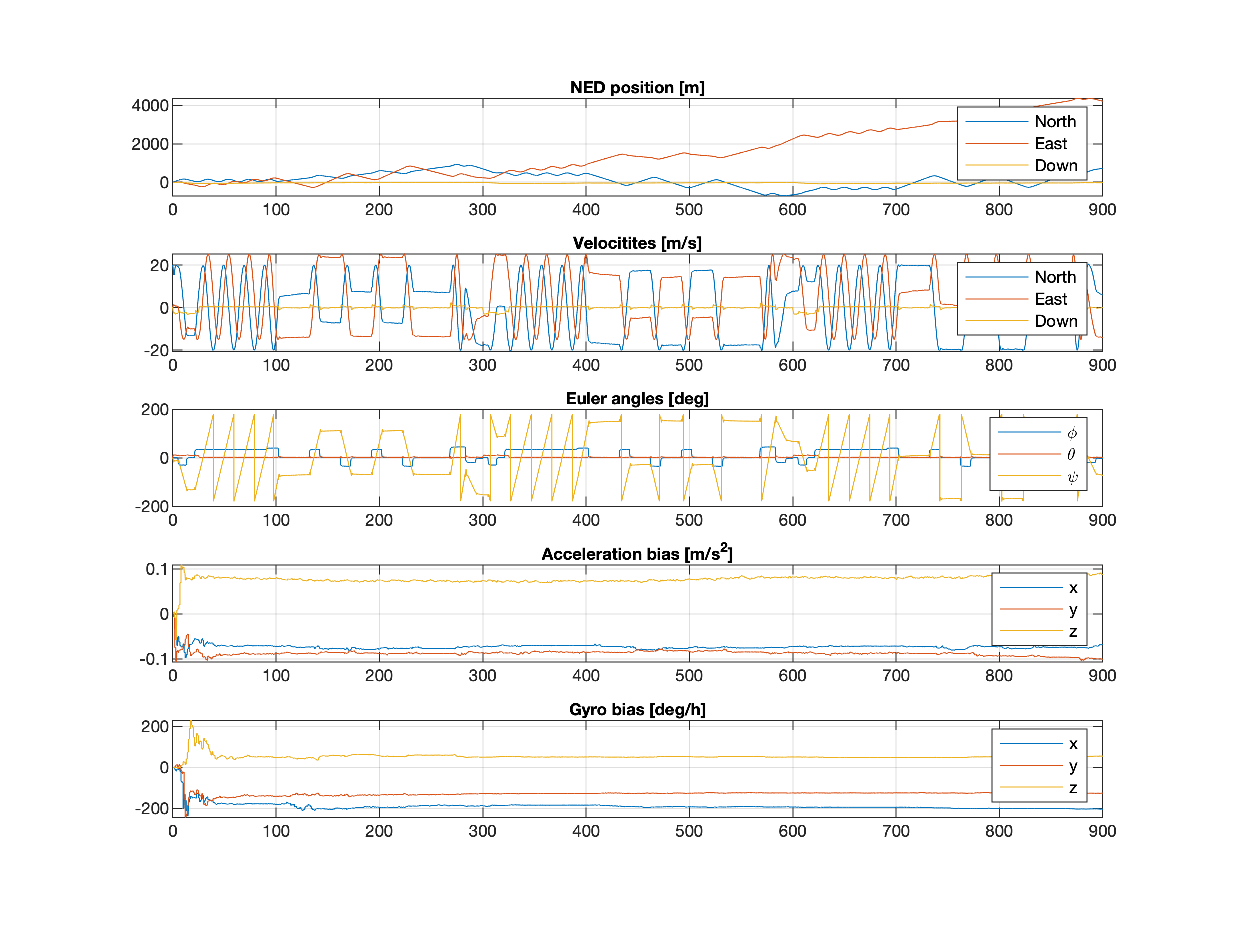
\includegraphics[width=\textwidth]{figures/ga_2/sim_state}
		\caption{UAV ESKF states}
		\label{fig:ga_2_sim_state}
	\end{subfigure}%
       ~
	\begin{subfigure}[b]{0.45\textwidth}
		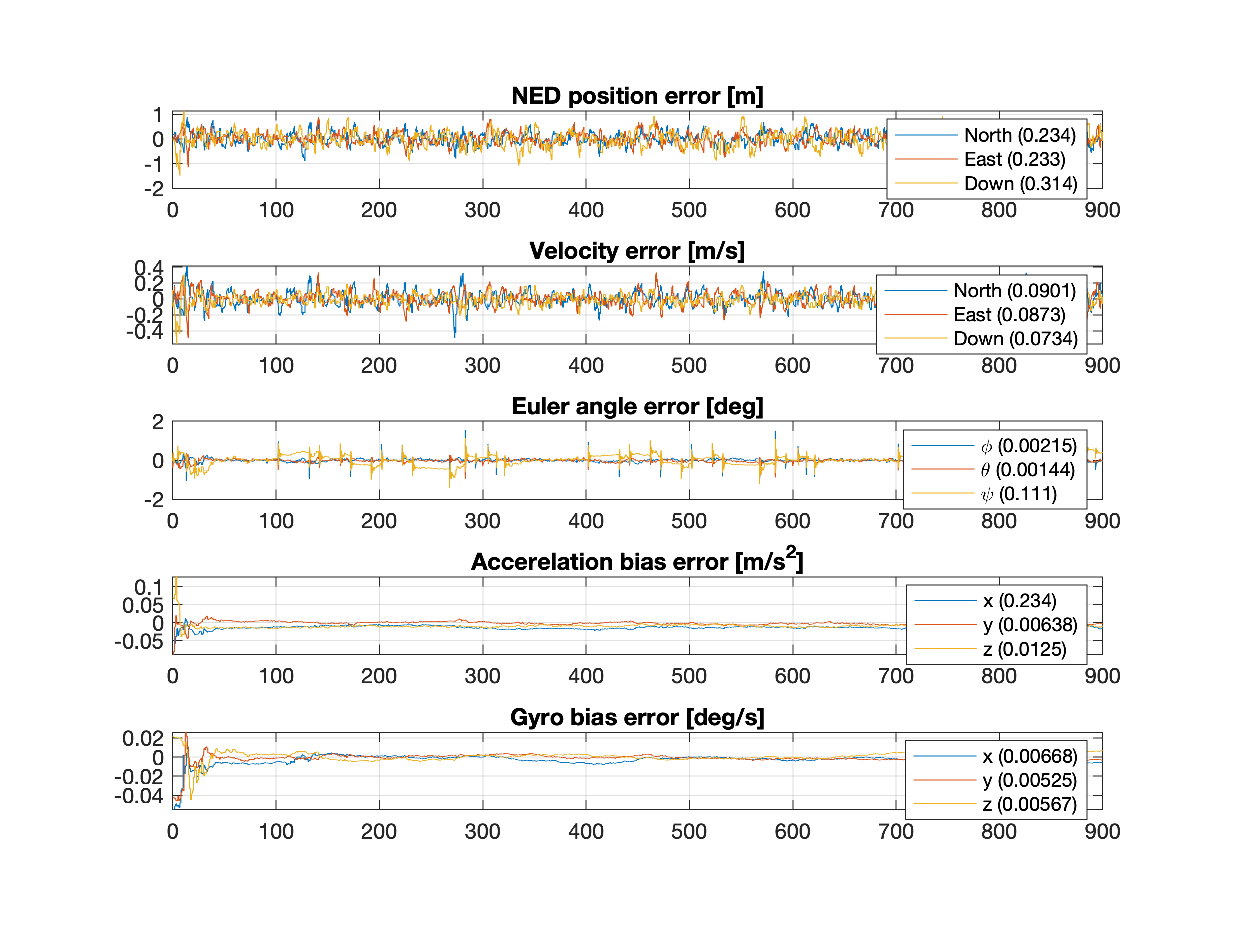
\includegraphics[width=\textwidth]{figures/ga_2/sim_errors}
		\caption{UAV ESKF state errors}
		\label{fig:ga_2_sim_errors}
    \end{subfigure}
    \caption{}
    \label{fig:ga_2_sim_state_errors} 
\end{figure}

\begin{figure}[ht]
    \centering
	\begin{subfigure}[b]{0.4\textwidth}
		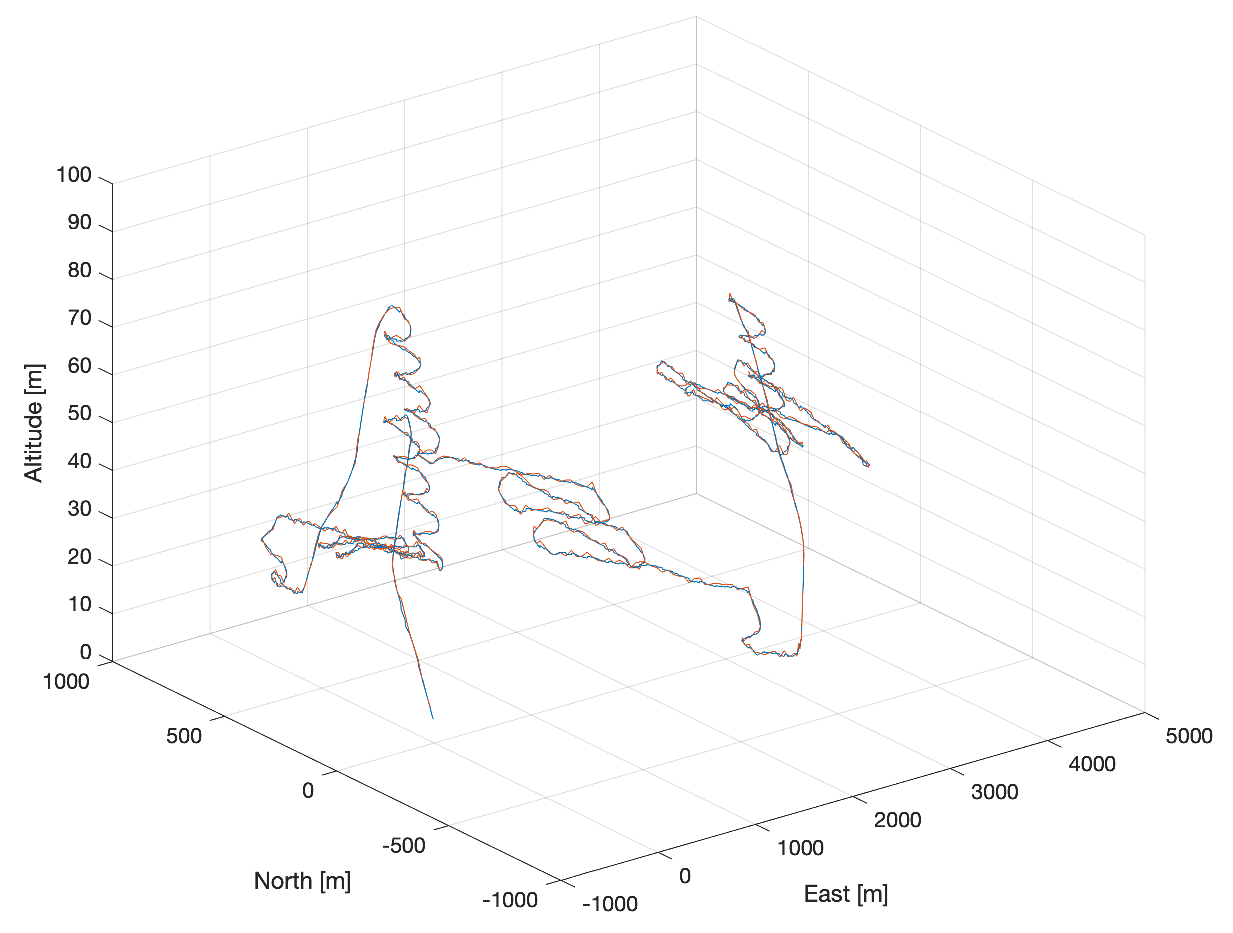
\includegraphics[width=\textwidth]{figures/ga_2/sim_trajectory.eps}
    \caption{Estimated UAV trajectory}
    \label{fig:ga_2_sim_trajectory}
	\end{subfigure}%
       ~
	\begin{subfigure}[b]{0.4\textwidth}
		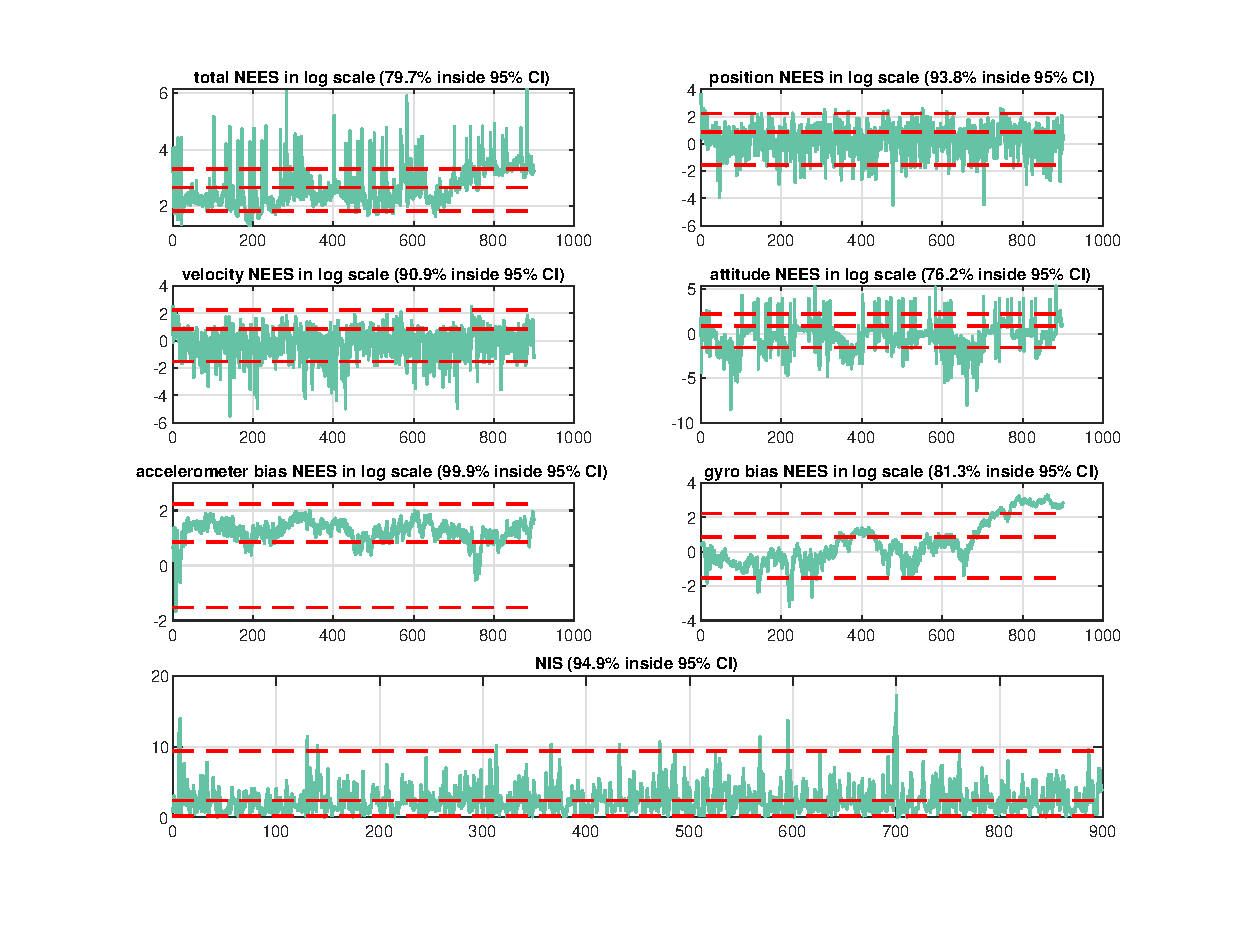
\includegraphics[width=\textwidth]{figures/ga_2/sim_consistency.eps}
    \caption{UAV ESKF consistency analysis}
    \label{fig:ga_2_sim_consistency}
    \end{subfigure}
    \caption{Estimated UAV trajectory and consistency analysis}
    \label{fig:ga_2_sim_trajectory_consistency} 
\end{figure}

The ESKF was in particular tuned such that the bias states converged nicely, such that the errors propagated in the system from sensor drift were minimised. It should be emphasised that one of the main features that makes the ESKF robust is the IMU bias estimation, and it was therefore also emphasised in the tuning process.

The consistency was also emphasised when tuning the ESKF. We see from \cref{fig:ga_2_sim_consistency} that most of the different normalized square errors are all in the 80\% or 90\% range inside the calculated confidence intervals, which was found to be satisfactory. One should especially note that the attitude NEES is only about 76\% inside the confidence interval. Studying the heading error in \cref{fig:ga_2_sim_errors} can give some insight into why this might be the lowest NEES. It is observed that the heading is at certain time intervals far off the ground truth, which is also confirmed by the RMSE of 0.111. This is about two magnitudes higher error than for pitch and roll. This is caused by the fact that pitch and roll are directly observable from the gravitational force acting on the accelerometer. Heading, on the other hand, is only observable when the system is exited by a manoeuvre. The heading error, therefore, has certain sections where it is unobservable and the update step is not able to correct the constant offset from the true value. This is further supported by studying the time intervals when the UAV is doing a spiral manoeuvre e.g. from about 300 to 400 seconds or from 600 to 700 seconds. In these intervals the heading is observable and as a consequence, we observe that the error drops to the same magnitude as the pitch and roll, before it starts acting unexpectedly again when the UAV starts flying straight. This issue might be why both the attitude NEES and total NEES is somewhat worse than the others. So the heading estimation would therefore not work if the UAV was standing still. 

When letting the sensor correction matrices be identity matrices, and thereby removing any sensor correction, the ESKF estimation performance is noticeably worse. While the filter is still able to reliably estimate velocity and position with the aid of the GNSS, the estimates of heading and sensor biases are much worse. Most importantly, the rate gyro and accelerometer biases no longer converge to the true sensor biases. This means we are not able to remove the bias in the measurements, and as a consequence, they are integrated and propagated through the Kalman filter. This makes all the RMSEs significantly worse, and especially the heading now drifts quickly when the UAV is not turning.

Another consequence is that the NEES and NIS also worsens significantly. While the position and velocity NEES is still somewhat within the confidence intervals at 85.2\% and 64.9\% respectively, the attitude, accelerometer bias and gyro bias is at 3.09\%, 14.6\% and 2.89\% respectively. This further supports the claim above about how important IMU bias compensation is when trying to design a robust attitude estimator. It is then evident that correction for sensor misalignment, scaling errors and orthogonality errors are a critical part of designing such an estimator. Neglecting the GNSS lever arm, on the other hand, has no noticeable effect on the estimator performance.

Finally, it must be said that finding the sensor correction matrices is not trivial, and the results will be empirically based and not absolutely correct. Therefore we will always have some sensor misalignment and miss-scaling in a physical system, especially since these matrices will, in reality, be time-varying.

\subsection{INS for real fixed-wing UAV}

% tuning a lot the same, but we started by looking at datasheet + simulated values. No NEES now, only NIS. Used GNSS accuracy thing. 

The ESKF was then tuned to a real data set from a fixed-wing UAV flight. The sensors on board was a STIM300 IMU and an u-blox M8 GNSS receiver. The GNSS receiver produces an accuracy estimate in standard deviation while operating. This was scaled by a gain parameter, squared and used as a time-varying GNSS measurement noise covariance signal. The gain was tuned to be $k_x = 0.5$.

The IMU measurement noise covariances and bias driving noise covariances were tuned from the Allan variances in the STIM300 datasheet \cite{stim300}. Specifically, the gyro noise and bias noise root Allan variance is \SI{0.15}{\deg\per\sqrt\hour} and \SI{0.5}{\deg\per\hour} respectively. The accelerometer noise and bias noise root Allan variance is \SI{0.06}{\meter\per\second\sqrt\hour} and \SI{0.05}{\meter g} respectively. These values were scaled to the correct units and used as initial parameters in the ESKF. The values were then tuned such that a satisfactory estimate and NIS were produced. The final tuning parameters were 
then $q_{a} = (\SI{9.8e-4})^2$, $ q_{ab} = (\SI{4.9e-4})^2$, $q_{\omega} = (\SI{4.9e-6})^2$ and $q_{\omega b} = (\SI{2.4e-6})^2$. When comparing to the simulated case, one sees that the bias noise standard deviations are of about the same magnitude, while the measurement noise standard deviations are about two magnitudes larger in the simulated case.

The resulting UAV trajectory estimate is presented in \cref{fig:ga_2_real_trajectory} and the estimated states are presented in \cref{fig:ga_2_real_state}. Finally the NIS is presented in \cref{fig:ga_2_real_consistency}. The average NIS was approximately 3.01. Note that since this is a real data set, we do no longer have the ground truth, and can therefore not calculate the estimation errors and NEES. This certainly makes tuning more challenging, even though access to the IMU datasheet is useful. This shows how it is often helpful to test filter implementations on simulated data first, as has been done in all of the assignments discussed in this report. The Gauss-Markov bias time constants were both tuned to $T_b = \SI{1e16}{s}$, effectively making the bias processes random walks processes.

\begin{figure}[ht]
    \centering
    \begin{subfigure}[b]{0.4\textwidth}
		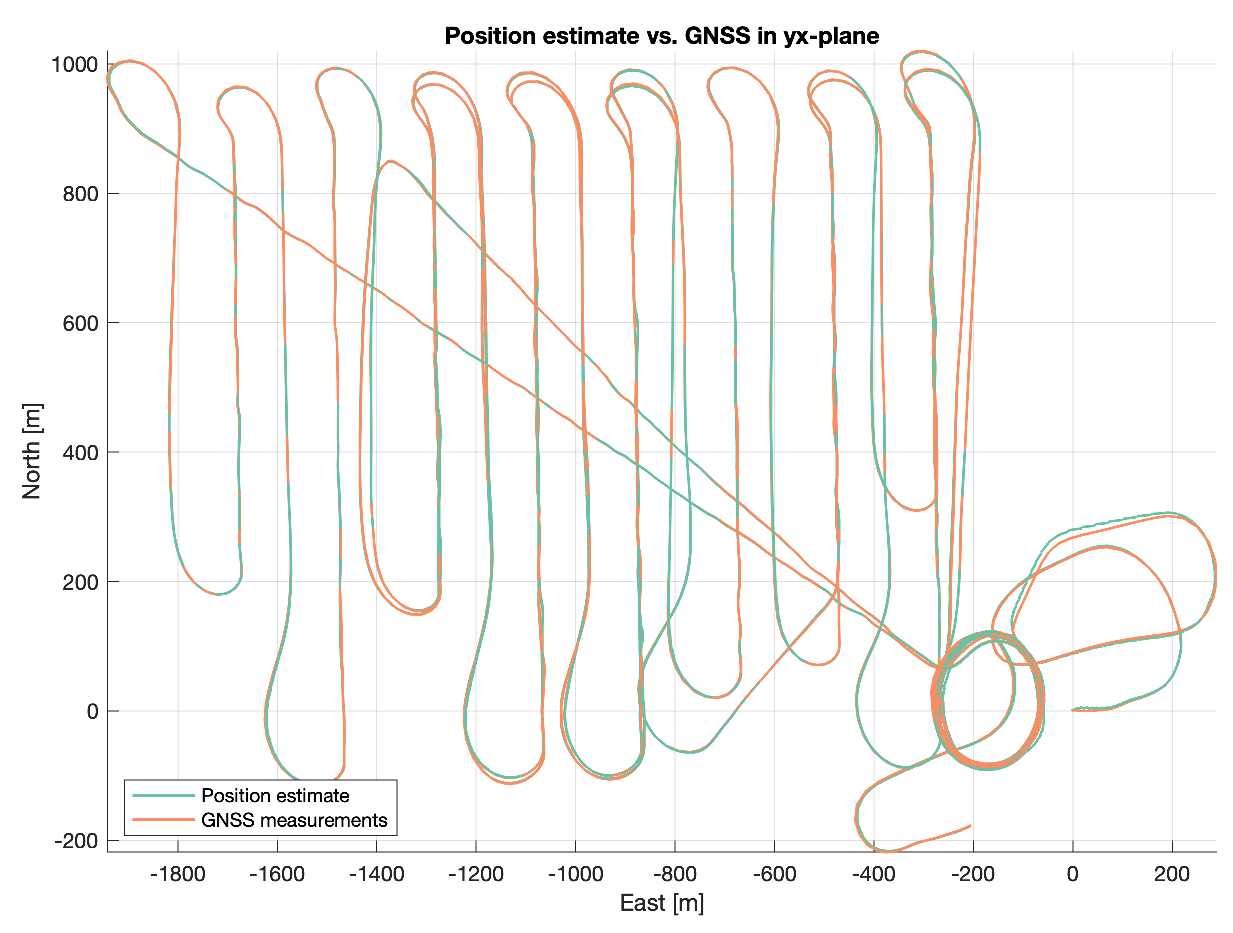
\includegraphics[width=\textwidth]{figures/ga_2/real_trajectory.eps}
        \caption{Estimated UAV trajectory}
        \label{fig:ga_2_real_trajectory}
	\end{subfigure}%
    \begin{subfigure}[b]{0.4\textwidth}
		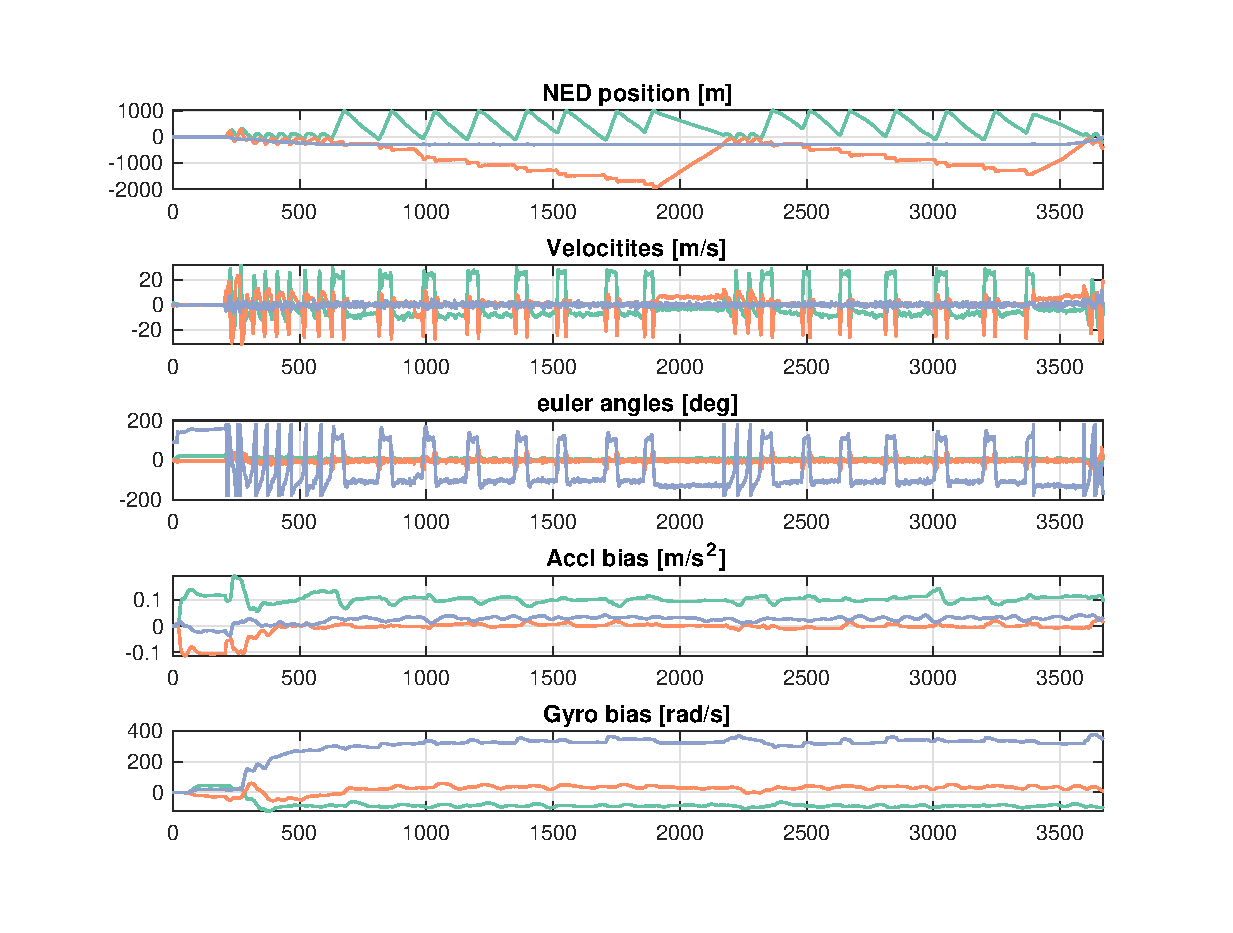
\includegraphics[width=\textwidth]{figures/ga_2/real_state.eps}
        \caption{UAV ESKF states}
        \label{fig:ga_2_real_state}
    \end{subfigure}
    \caption{}
    \label{fig:ga_2_real_trajectory_state}
\end{figure}

\begin{figure}[!htb]
    \centering
    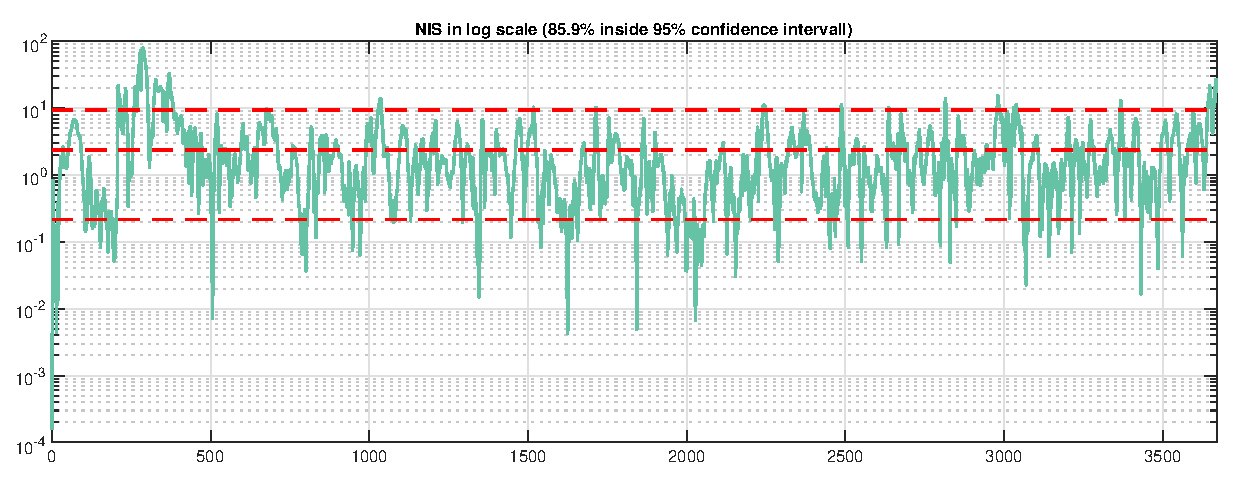
\includegraphics[width=0.7\linewidth]{figures/ga_2/real_consistency.eps}
    \caption{UAV GNSS logarithmic NIS}
    \label{fig:ga_2_real_consistency}
\end{figure}

We observe how the estimated trajectory fits nicely with the GNSS data as one would expect. The estimates are also nicely behaved, while the state trajectories are naturally a lot less smooth in this case compared to the simulation, which is to be expected. In particular, the biases converge over time, with some corrections throughout the flight when the UAV turns and the system is excited. From the heading plot it seems like the bias estimates work well, as there is no noticeable drift in heading. For most of the flight, we see that the heading changes between two almost constant values. This is reflected by the UAV manoeuvres in \cref{fig:ga_2_real_trajectory}, where the UAV flies straight north, then quickly does a U-turn, then flies straight south, then does a U-turn and so on. 

When the sensor correction matrices were set to identity for the real data, it was observed again that thanks to the GNSS measurements the position and velocity estimates are still viable. But the biases do not converge to the same values as before. Interestingly, the heading is now mirrored around zero, and the roll and pitch estimates are \textit{swapped}, as can be seen in \cref{fig:ga_2_real_bad}. This is due to the fact that the sensor frame is no longer approximately aligned with the body frame. While in the simulated case the sensor correction matrices were close to identity, for this data set they are
\begin{equation}
    S_g = \begin{bmatrix}
        -0.0243 & 0.9981  & 0.0454 \\
        -0.9998 & -0.0242 & -0.0255 \\
        -0.0272 & -0.0532 & 0.9949
    \end{bmatrix}, \quad
    S_a = \begin{bmatrix}
        -0.0503 & 1.0021  & 0.0476 \\
        -1.0243 & -0.0695 & -0.0197 \\
        -0.0387 & -0.0483 & 1.0005
    \end{bmatrix}.
\end{equation}
Now notice that $S_g \approx R_z(-\frac{\pi}{2}), S_a \approx R_z(-\frac{\pi}{2})$. This means that in addition to small scaling, misalignment and orthogonality errors there is a \SI{90}{\degree} rotation that is needed in order to convert the measurements from sensor to body frame. When implementing an ESKF, and even more generally some sensor fusion algorithm in a physical application such as this, one obviously needs to consider that very rearily will sensors be mounted along the body axes, and a sensor to body transformation is therefore absolutely necessary for the system to work. Luckily, it is easy to see from the estimates or even the measurements themselves that they do not correspond to what common sense it telling you e.g. in this case that the heading estimate points southwards when the plane is flying north and vice-versa. 

\begin{figure}[!htb]
    \centering
    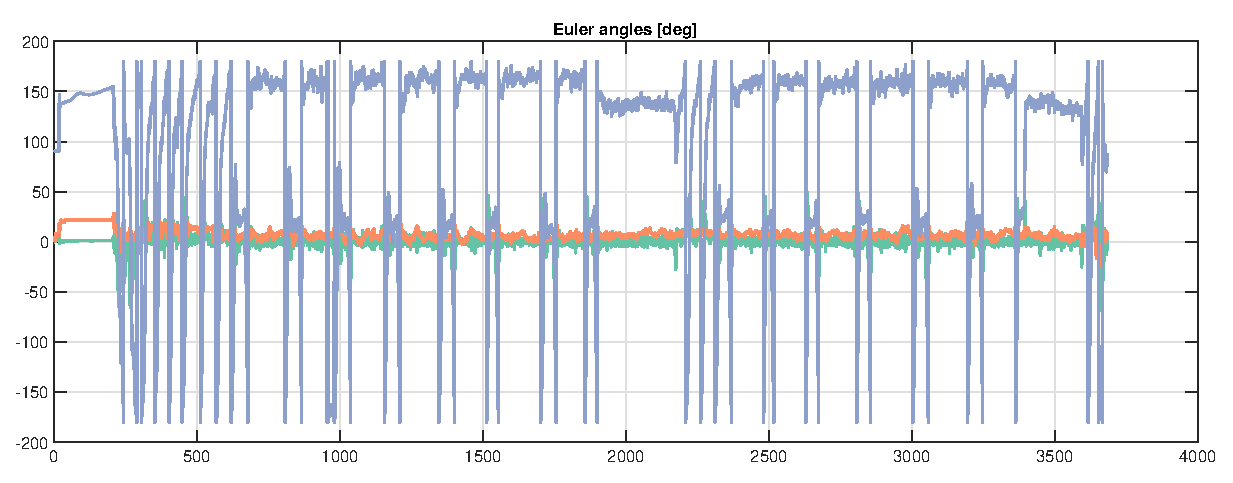
\includegraphics[width=0.6\linewidth]{figures/ga_2/real_bad_heading.eps}
    \caption{UAV estimated attitude without sensor error correction}
    \label{fig:ga_2_real_bad}
\end{figure}

% discuss assumptions, linearity, convergence - knowing initial values? Robustness

One could argue that the benefits of the ESKF are twofold. Firstly, since the error dynamics are approximately linear, the optimality of the linear Kalman filter, which is lost when extending it to non-linear process and measurement models with the EKF, are (approximately) retained. Secondly, since the IMU is treated as a control input and the IMU biases are estimated, we achieve robustness, as has previously been discussed. In the test implementations in this assignment, with both simulated and real data sets, this has been observed. By masking modelling errors, sensor errors, uncertainties and actual sensor biases within these states, the filter system is able to operate in a dynamic environment where the plant performs various different manoeuvres, even with wind disturbance and temperature fluctuations.

One could argue that the main limitation of the ESKF for inertial navigation is its slow convergence for deficient initial attitude values. In these tests of the filter, this has not been an issue, as good initial values were provided. One should note that this is not always the case. In many real-time applications, you cannot expect to turn on your INS and have good initial estimates of the attitude. If one tries to give an arbitrary attitude initialization to the ESKF, one observes poor estimates that are not at all usable. Due to length limitations this cannot be further explored here, but nevertheless this is a problem that could be further analysed and extensions to the ESKF could be added to handle this e.g. with optimization methods.